\chapter{Problema dei cammini minimi - Floyd-Warshall}
Come al solito diamo qualche definizione per poter lavorare successivamente in maniera
agile.
\section{Definizioni}
\subsection{Grafo}
Un Grafo viene definito come $G=(V,E)$ dove:
\begin{itemize}
    \item $V = \{v_1,v_2,v_3,...,v_n\}$ insieme di vertici
    \item $E= \{e_1,e_2,e_3,...,e_m\}$ insieme di archi
\end{itemize}
\paragraph*{Dimensione di G} $\rightarrow$ (n,m).
Arco $e_k \rightarrow$ relazione R tra due vertici $v_i$ e $v_j$
\paragraph*{R può essere}
\begin{itemize}
    \item Simmetrica - Grafo NON Orientato - cioè $v_i \, R \, v_j \Leftrightarrow v_j \, R \, v_i$
    \item Asimmetrica - Grafo Orientato (o diretto) - cioè $v_i \, R \, v_j \nLeftrightarrow  v_j \, R \, v_i$
\end{itemize}
Un grafo orientato è caratterizzato da un verso di percorrenza degli archi unidirezionale.
In questo caso E è sottoinsieme di $V^2$.
\begin{center}
    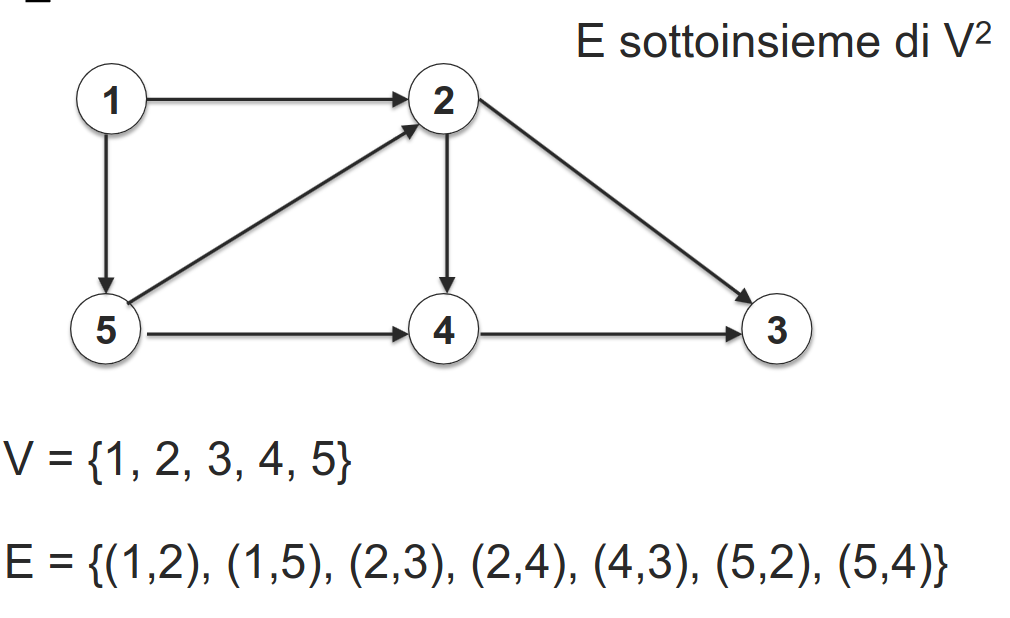
\includegraphics[width=80mm, scale=0.5]{grafo_orientato.png}
\end{center}
\begin{center}
    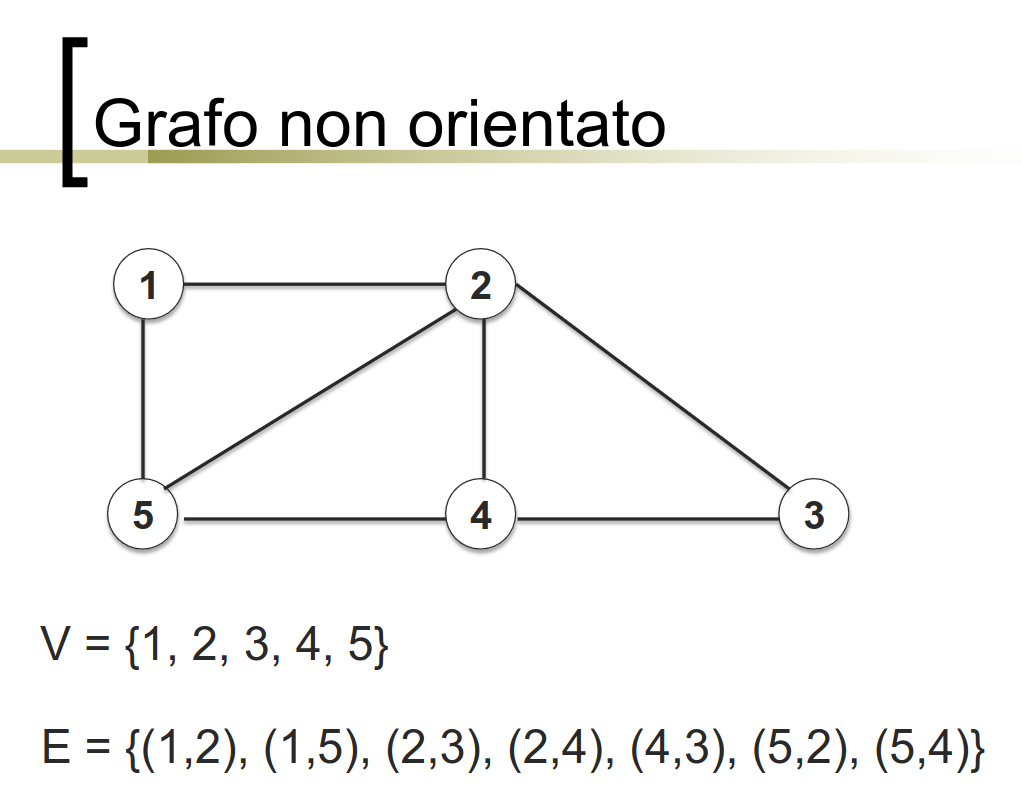
\includegraphics[width=80mm, scale=0.5]{grafo_non_orientato.png}
\end{center}
\subsection{Adiacenza}
Un vertifica v è adiacente a un vertice u se $(u,v)\in E$.\\
Per esempio nella rappresentazione del grafo orientato il vertice \textbf{1} è adiacante ai
vertici \textbf{2 e 5}, infatti notiamo che in E è presente $(1,2), (1,5)$.
\subsection{Rappresentazione di un grafo}
Abbiamo 2 rappresentazioni possibili:
\begin{itemize}
    \item Liste di adiacenza
    \item Matrice di adiacenza
\end{itemize}
\begin{enumerate}
    \item Le liste di adiacenza utilizzano un vettore $L_v$ di dimensione $|V|$ tale che $V[i]$ è la lista degli
    adiacenti del vertice $v_i$. Ogni vertice del grafo avrà un vettore.
    \item La matrice di adiacenza è una Matrice $M_v$ di dimensione $n \times n$ tale che $M[i,j] = 1$ se il
    vertice j è adiacente del vertice i, altrimenti $M[i,j] = 0$. A differenza delle liste in questo caso ho una sola
    matrice.
\end{enumerate}
\subsection{Esempio grafo orientato}
\begin{center}
    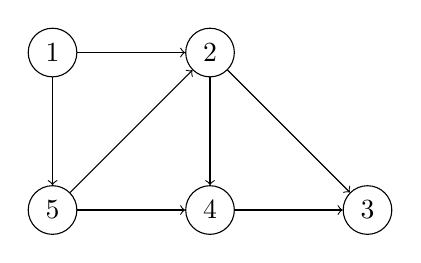
\begin{tikzpicture}
        \node[shape=circle,draw=black] (1) at (0,0) {1};
        \node[shape=circle,draw=black] (2) at (2,0) {2};
        \node[shape=circle,draw=black] (3) at (4,-2) {3};
        \node[shape=circle,draw=black] (4) at (2,-2) {4};
        \node[shape=circle,draw=black] (5) at (0,-2) {5};

        \path [->] (1) edge node[left] {} (2);
        \path [->] (2) edge node[left] {} (3);
        \path [->] (1) edge node[left] {} (5);
        \path [->] (5) edge node[left] {} (2);
        \path [->] (2) edge node[left] {} (4);
        \path [->] (5) edge node[left] {} (4);
        \path [->] (4) edge node[left] {} (3);

    \end{tikzpicture}
\end{center}

\begin{equation*}
    M = \begin{array}{c|ccccc}
    & 1 & 2 & 3 & 4 & 5 \\
    \hline
    1 & 1 & 0 & 0 & 1 & 0 \\
    2 & 0 & 0 & 1 & 1 & 0 \\
    3 & 0 & 0 & 0 & 0 & 0 \\
    4 & 0 & 1 & 0 & 0 & 0 \\
    5 & 1 & 0 & 1 & 0 & 0 \\
    \end{array}
\end{equation*}
\paragraph*{Dimensione} $|V|^2=n^2$
\paragraph*{Numero di celle con 1} $|E|$

\subsection{Esempio grafo non orientato}
\begin{center}
    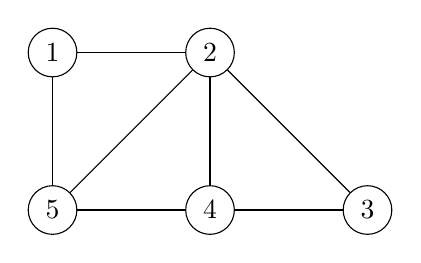
\begin{tikzpicture}
        \node[shape=circle,draw=black] (1) at (0,0) {1};
        \node[shape=circle,draw=black] (2) at (2,0) {2};
        \node[shape=circle,draw=black] (3) at (4,-2) {3};
        \node[shape=circle,draw=black] (4) at (2,-2) {4};
        \node[shape=circle,draw=black] (5) at (0,-2) {5};

        \path [-] (1) edge node[left] {} (2);
        \path [-] (2) edge node[left] {} (3);
        \path [-] (1) edge node[left] {} (5);
        \path [-] (5) edge node[left] {} (2);
        \path [-] (4) edge node[left] {} (2);
        \path [-] (5) edge node[left] {} (4);
        \path [-] (4) edge node[left] {} (3);

    \end{tikzpicture}
\end{center}

\begin{center}
    \begin{equation*}
        M = \begin{array}{c|ccccc}
          & 1 & 2 & 3 & 4 & 5 \\
        \hline
        1 & 0 & 1 & 0 & 0 & 1 \\
        2 & 1 & 0 & 1 & 1 & 1 \\
        3 & 0 & 1 & 0 & 1 & 0 \\
        4 & 0 & 1 & 1 & 0 & 1 \\
        5 & 1 & 1 & 0 & 1 & 0 \\
        \end{array}
        \end{equation*}
\end{center}
\paragraph*{Dimensione} $|V|^2=n^2$
\paragraph*{Numero di celle con 1} $2|E|$
\subsection{Liste VS Matrice (memoria)}
\paragraph*{Liste di adiacenza} Sono ottime dal punto di vista dell'occupazione dello spazio 
nel caso di Grafi sparsi con $|E|$ molto minore di $|V|^2$.
\paragraph*{Matrici di adiacenza} Risultano migliori nei grafi densi quindi quando ho
$|E|$ che si avvicina a $|V|^2$.
\subsection{Liste VS Matrice (tempo)}
\paragraph*{(u,v)} Intendiamo se i 2 vertici sono collegati.
Come tempo intendiamo il tempo per stabilire se (u,v) appartiene ad E e i tempi
sono i seguenti:
\begin{itemize}
    \item Liste di adiacenza $\rightarrow O(|E|) = O(m)$
    \item Matrice di adiacenza $\rightarrow O(1)$
\end{itemize}
\subsection{Cammino in un grafo orientato}
\paragraph*{Definizione di cammino} Sequenza $P=<v_{i_1},v_{i_2},..., v_{i_{k-1}},v_{i_k}>$
tale che $v_{i_k}$ appartiene a V per $1\leq j \leq k$ e $(v_{i_j},v_{i_{j+1}})$ appartiene
ad E per $1 \leq j < k$.
